%%%%%%%%%%%%%%%%%%%%%%%%%%%%%%%%%%%%%%%%%%%%%%
%                insertmeeting
% 1) Title (something creative & funny?)
% 2) Date (MM/DD/YYYY)
% 3) Location (ex. Hagerty High School)
% 4) People/Committees Present 
% 5) Picture 
% 6) Start Time & Stop Time (ex. 12:30AM to 4:30PM)
%%%%%%%%%%%%%%%%%%%%%%%%%%%%%%%%%%%%%%%%%%%%%%
\insertmeeting 
	{(Past) April Fools Autonomous} 
	{04/05/22} 
	{Hagerty High School}
	{James, Jensen, Nathan, Ritam}
	{Images/RobotPics/robot.jpg}
	{2:30 - 4:30}
	
\hhscommittee{Software}
\noindent\hfil\rule{\textwidth}{.4pt}\hfil
\subsubsection*{Goals}
\begin{itemize}
    \item Fine tune some parts of autonomous.

\end{itemize} 

\noindent\hfil\rule{\textwidth}{.4pt}\hfil

\subsubsection*{Accomplishments}
In today's relatively shorter meeting, we mainly focused on running the autonomous to ensure its consistency. We tried a variety of adjustments, such as tiny variations in the starting location and some changes in trajectories. But other than that, most of our autonomous code was just tested today for consistency. It worked pretty well. After that, we handed the robot over to the driveteam for driver practice. 


\begin{figure}[htp]
\centering
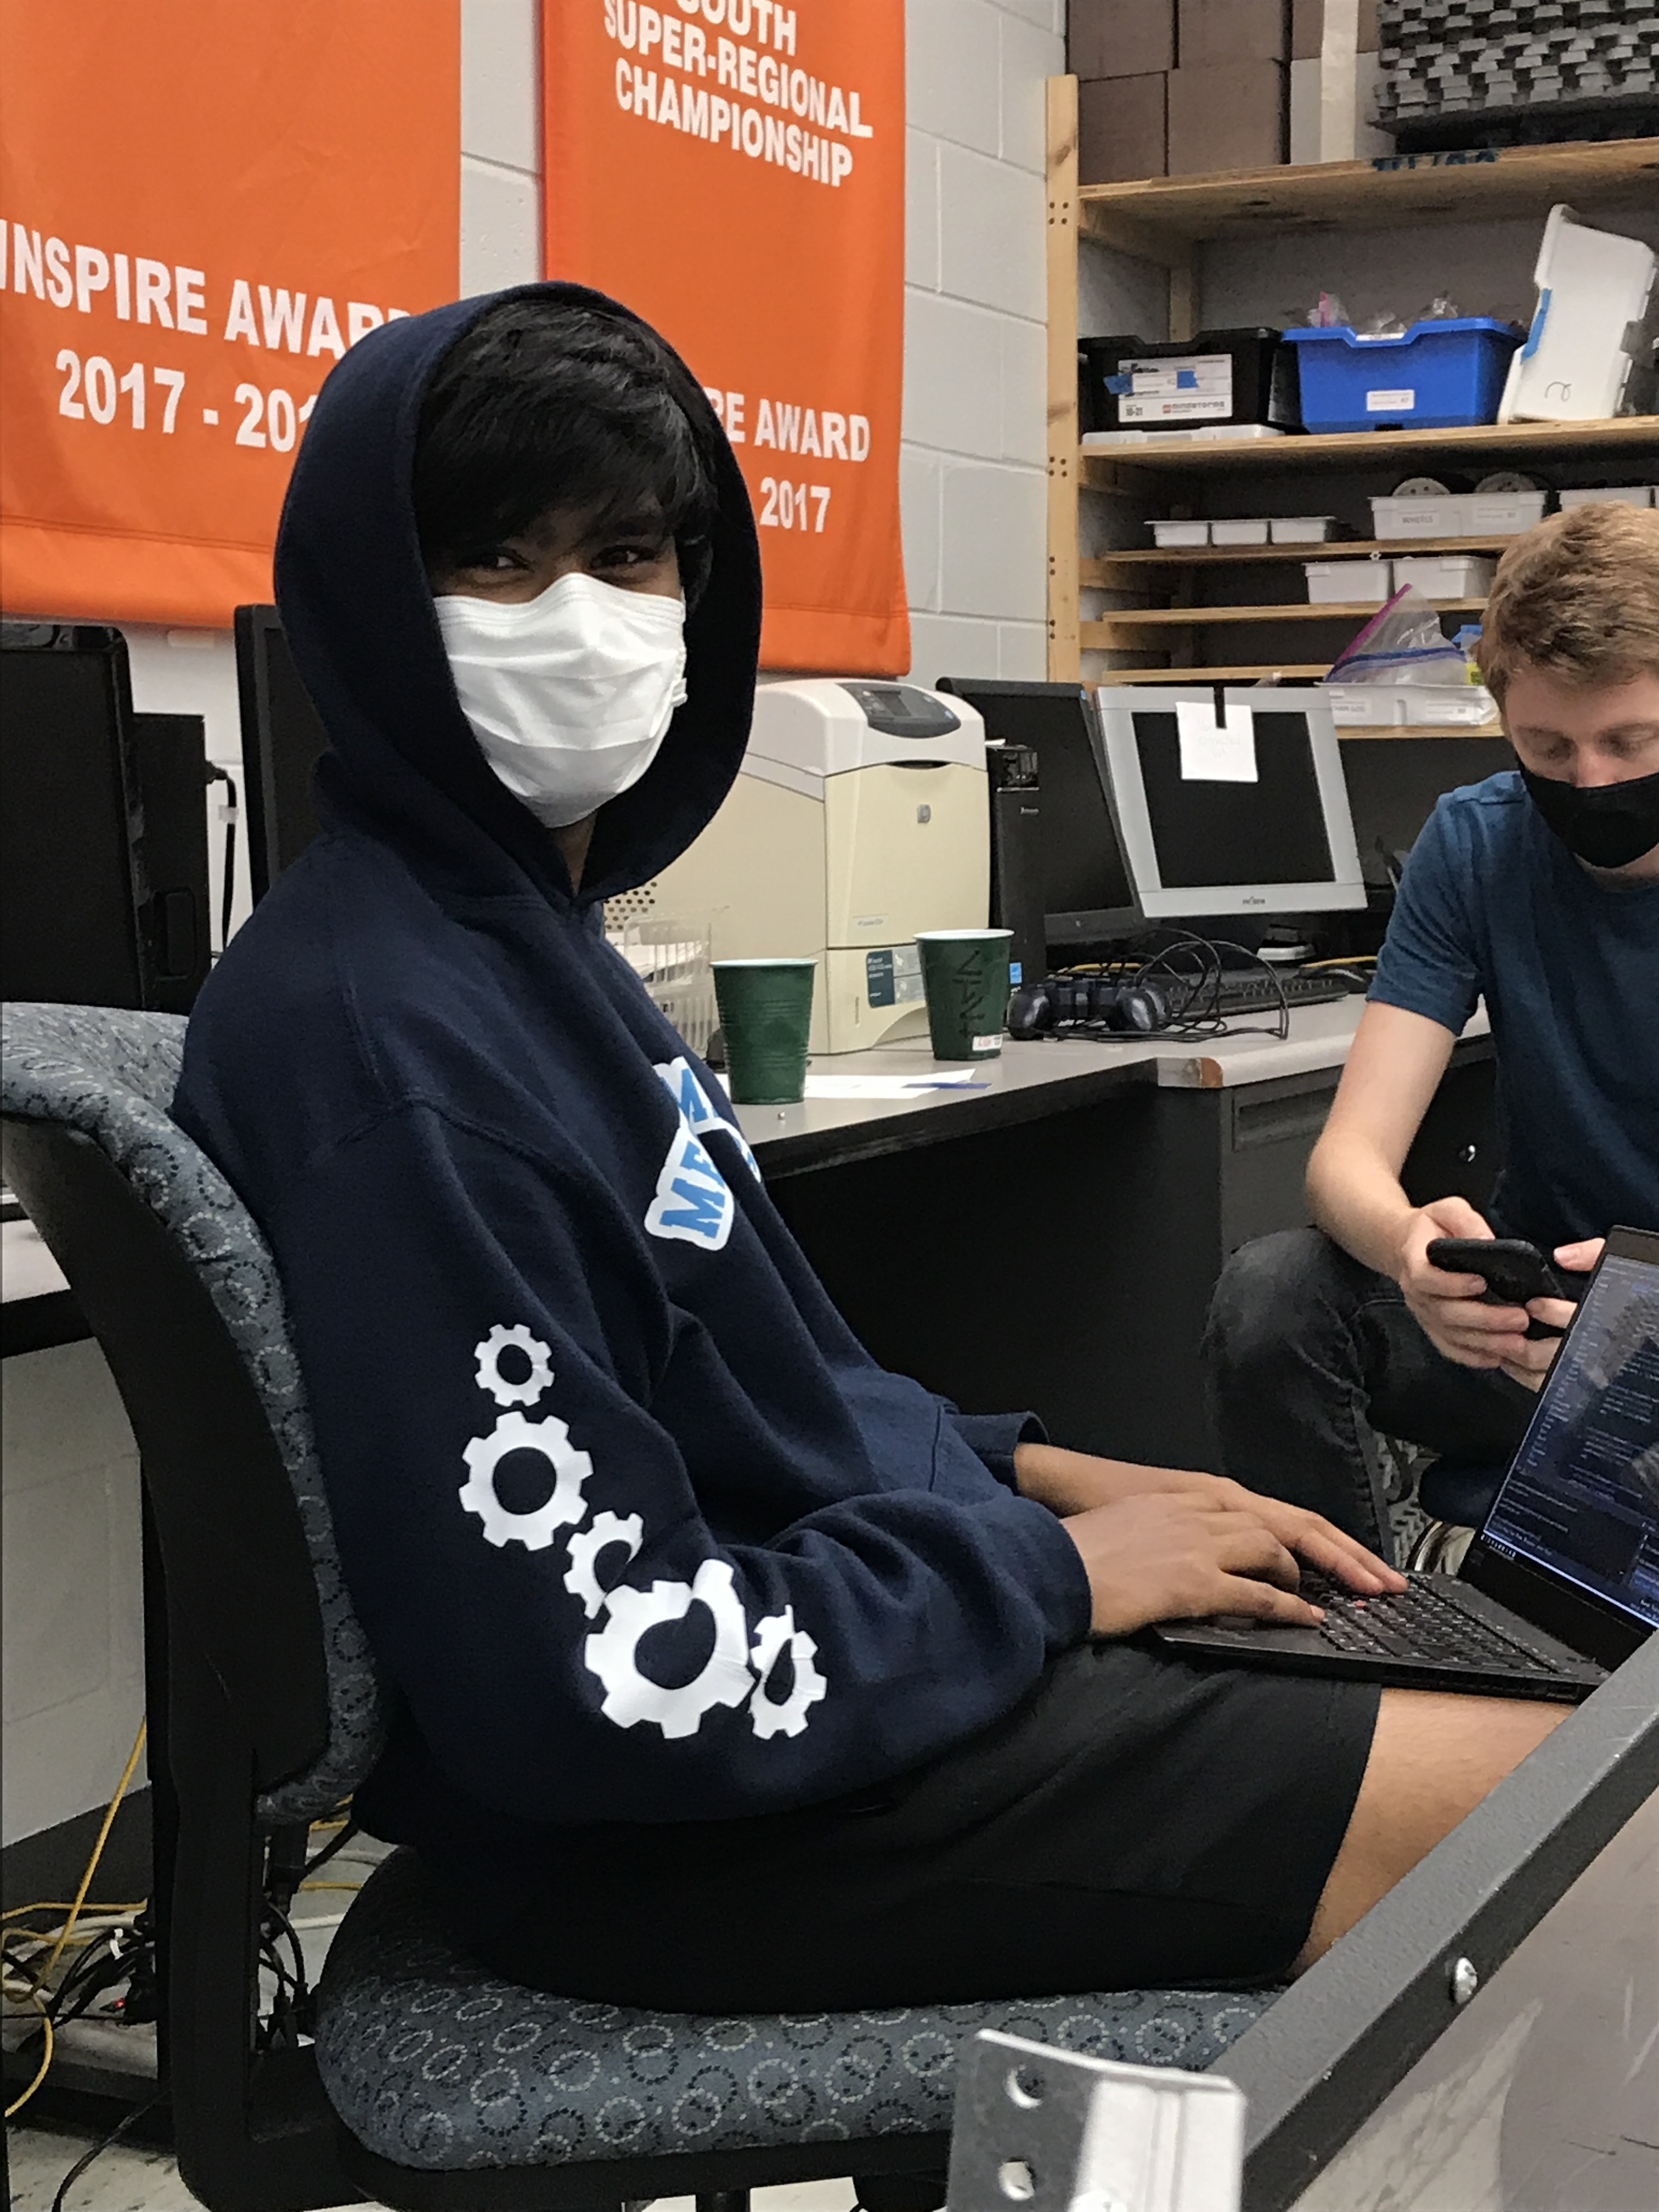
\includegraphics[width=0.95\textwidth, angle=0]{Meetings/April/04-05-22/04-05-22 1.JPG}
\caption{Ritam hard at work testing our autonomous programs.}
\label{fig:040522_1}
\end{figure}



\whatsnext{
\begin{itemize}
    \item Get the autonomous ready for Worlds while giving the drivers time to practice.
\end{itemize} 
}

